\documentclass[11pt]{article}
\usepackage[margin=1in]{geometry}
\usepackage{booktabs}
\usepackage{graphicx}
\usepackage{amsmath,amssymb}
\usepackage{hyperref}
\usepackage{natbib}
\usepackage{xcolor}
\usepackage{microtype}
\graphicspath{{../figures/}}
\newcommand{\ResolveQwenTwoXFiveXOneXFivebUngoverned}{18.8\%}
\newcommand{\ScoreQwenTwoXFiveXOneXFivebUngoverned}{0.592}
\newcommand{\GovQwenTwoXFiveXOneXFivebUngoverned}{n/a}
\newcommand{\ReviewsQwenTwoXFiveXOneXFivebUngoverned}{2}
\newcommand{\ResolveQwenTwoXFiveXOneXFivebVerified}{18.8\%}
\newcommand{\ScoreQwenTwoXFiveXOneXFivebVerified}{0.592}
\newcommand{\GovQwenTwoXFiveXOneXFivebVerified}{n/a}
\newcommand{\ReviewsQwenTwoXFiveXOneXFivebVerified}{2}
\newcommand{\ResolveQwenTwoXFiveXOneXFivebGoverned}{33.3\%}
\newcommand{\ScoreQwenTwoXFiveXOneXFivebGoverned}{0.663}
\newcommand{\GovQwenTwoXFiveXOneXFivebGoverned}{0/15}
\newcommand{\ReviewsQwenTwoXFiveXOneXFivebGoverned}{16}
\newcommand{\ResolveQwenTwoXFiveXOneXFivebFdeDisciplined}{22.9\%}
\newcommand{\ScoreQwenTwoXFiveXOneXFivebFdeDisciplined}{0.537}
\newcommand{\GovQwenTwoXFiveXOneXFivebFdeDisciplined}{0/15}
\newcommand{\ReviewsQwenTwoXFiveXOneXFivebFdeDisciplined}{22}
\newcommand{\FriedmanP}{0.0753}
\newcommand{\MarketPostings}{3,473}
\newcommand{\MarketFDE}{670}
\newcommand{\MarketFDEShare}{19.3\%}
\newcommand{\MarketExplicit}{229}
\newcommand{\MarketExplicitShare}{6.6\%}
\newcommand{\MarketExplicitOfFDE}{34.2\%}
\newcommand{\SalaryN}{205}
\newcommand{\SalaryShare}{30.60\%}
\newcommand{\SalaryMedianLow}{\$182,000}
\newcommand{\SalaryMedianHigh}{\$182,000}
\newcommand{\GuardRecall}{95.1\%}
\newcommand{\GuardPrecision}{65.2\%}
\newcommand{\LambdaGBSecond}{1.33334e-05}
\newcommand{\TaskRows}{48}
\newcommand{\TaskTemplates}{6}
\newcommand{\DistinctInstructions}{13}
\newcommand{\VerifiedPairs}{48}
\newcommand{\VerifiedNonErrorPairs}{46}
\newcommand{\VerifiedChanged}{0}
\newcommand{\VerifiedImproved}{0}
\newcommand{\VerifiedWorse}{0}
\newcommand{\VerifiedIdentical}{42}
\newcommand{\VerifiedIdenticalNonError}{40}
\newcommand{\VerifiedBothError}{2}
\newcommand{\FdePairs}{48}
\newcommand{\FdeChanged}{23}
\newcommand{\FdeImproved}{8}
\newcommand{\FdeWorse}{15}
\newcommand{\FdeIdentical}{0}
\newcommand{\FdeIdenticalNonError}{0}
\newcommand{\FdeBothError}{0}
\newcommand{\RepairEpisodes}{37}
\newcommand{\GovHighRiskPerfectUnresolved}{11}
\newcommand{\DeployTotal}{32}
\newcommand{\DeployValidCompose}{1}


% Short aliases for the single reported model. The generated names are
% letters-only because TeX control words cannot contain digits.
\newcommand{\ResolveUngoverned}{\ResolveQwenTwoXFiveXOneXFivebUngoverned}
\newcommand{\ResolveVerified}{\ResolveQwenTwoXFiveXOneXFivebVerified}
\newcommand{\ResolveGoverned}{\ResolveQwenTwoXFiveXOneXFivebGoverned}
\newcommand{\ResolveDisciplined}{\ResolveQwenTwoXFiveXOneXFivebFdeDisciplined}
\newcommand{\GovUngoverned}{\GovQwenTwoXFiveXOneXFivebUngoverned}
\newcommand{\GovVerified}{\GovQwenTwoXFiveXOneXFivebVerified}
\newcommand{\GovGoverned}{\GovQwenTwoXFiveXOneXFivebGoverned}
\newcommand{\GovDisciplined}{\GovQwenTwoXFiveXOneXFivebFdeDisciplined}

\title{Forward-Deployed Engineering for Enterprise AI Agents:\\[0.4em]
A Measurement Study and a Null Result for Check-Driven Repair}
\author{AI FDE Research}
\date{October 2026}

\begin{document}
\maketitle

\begin{abstract}
Forward-deployed engineering (FDE) is a delivery model for enterprise AI agents, but its evidence base is thin. We report a point-in-time snapshot of \MarketPostings{} public job postings, a \TaskRows{}-row benchmark of FDE deliverables, a four-policy comparison on a small local model, a prompt-injection guardrail evaluation, and a shadow-price cost model. The benchmark is not \TaskRows{} independent scenarios: it is \TaskTemplates{} templates with eight parameterizations each, and five phases reuse one instruction across all eight parameterizations (\DistinctInstructions{} distinct instruction strings in total). The model sees the acceptance criteria, so the benchmark measures instruction-following against explicit rubrics, not hidden FDE capability.

The main result is a null result. One repair attempt driven by failed checks changed \VerifiedChanged{} of \VerifiedPairs{} scores; \VerifiedIdenticalNonError{} non-error pairs were byte-identical; \VerifiedBothError{} additional pairs were both errors. The ungoverned and verified policies both resolved \ResolveUngoverned{} and \ResolveVerified{} of tasks. Governed and disciplined policies are reported with task resolution and governance compliance as separate outcomes: \ResolveGoverned{} task-resolved with \GovGoverned{} compliance, and \ResolveDisciplined{} task-resolved with \GovDisciplined{} compliance, where compliance is measured among required high-risk episodes. \GovHighRiskPerfectUnresolved{} governed or disciplined high-risk episodes passed every check while omitting the approval field. We do not claim four-policy superiority, verification gains, or that generated deployment stacks run. The contribution is a reproducible measurement protocol and a negative result: check-driven repair did not move outcomes in this task bank, and task resolution must not be conflated with governance compliance.
\end{abstract}

\section{Introduction}
Enterprise AI agents are sold as outcomes, but they are delivered as engineering projects inside a customer's environment. The person who does that work is increasingly called a forward-deployed engineer (FDE): part solutions architect, part software engineer, part security reviewer, part change manager. The role is not new---Palantir popularized it---but the 2025--2026 generative-AI cycle turned it into a labor-market category. Lightcast observed roughly 200 US postings in 2024, about 1,200 in 2025, and more than 5,200 in the first seven months of 2026 \citep{lightcast2026}. A CNBC analysis counted 7,300 US postings in the first nine months of 2026 and a median advertised salary of \$195,456 \citep{cnbc2026}. Vendors are investing directly: Anthropic announced \$100M to train 10,000 FDEs by the end of 2027, AWS announced a \$1B deployment initiative, and OpenAI scaled a multi-billion-dollar deployment business \citep{cnbc2026}.

Growth has outpaced evidence. The FDE Jobs 2026 report finds that 83\% of FDE-like postings do not use the title, which makes naive keyword counts unreliable \citep{fdejobs2026}. Practitioner accounts describe the lifecycle---discovery, architecture, security review, context assembly, deployment, handover---but rarely measure which phase breaks \citep{cio2026}. FDE-Bench introduced 136 deployment-configuration tasks with 2,145 checks and showed that frontier models resolve 52.9--75.0\% of them, with readiness the largest failure category \citep{fdebench2026}. That benchmark is an important start, but it covers one phase. An FDE is judged across the whole engagement: a perfect Compose file does not compensate for a missed approval gate or an ungrounded retrieval design.

This paper asks five questions. RQ1: what does the 2026 market ask of FDE-like roles, and how sensitive is the count to the title definition? RQ2: which lifecycle phases are hardest for a small open-weight model under explicit acceptance criteria? RQ3: do verification, approval gates, and a disciplined delivery loop change task outcomes or governance compliance? RQ4: how well do lightweight guardrails detect prompt injection in customer content? RQ5: do canonical and generated deployment artifacts run, and what does governance cost per resolved task?

Our contributions are:
\begin{enumerate}
\item A reproducible point-in-time labor-market snapshot of \MarketPostings{} public postings, with a broad FDE-like class and an explicit \texttt{forward deployed} sensitivity count.
\item FDE-LifecycleBench: \TaskRows{} rows across six phases, explicit acceptance criteria, and reference artifacts that pass their own checks. We also document that the rows are \TaskTemplates{} templates with eight parameterizations each, which limits the effective sample size.
\item A four-policy measurement on one local open-weight model, reporting task resolution, governance compliance, partial score, safety violations, and review burden as separate outcomes.
\item A guardrail evaluation, a canonical-only deployment smoke test, and a shadow-price cost model. We do not claim that generated deployment stacks execute.
\item A freeze-before-analysis protocol, a schema that separates task and governance outcomes, and code that regenerates every local number (external sources are cited, not re-estimated).
\end{enumerate}

\section{Background and related work}
\paragraph{The FDE role.} FDEs are embedded engineers who own the customer outcome rather than a product surface. Practitioner guides emphasize discovery, executive communication, and the ability to ship inside constraints the customer did not document \citep{cio2026}. The role overlaps with solutions engineering, professional services, and platform engineering, which is why title-based measurement undercounts it \citep{fdejobs2026}.

\paragraph{Deploying machine learning.} The ML systems literature has long argued that deployment, monitoring, and organizational ownership dominate model quality \citep{sculley2015,paleyes2022}. Production-readiness rubrics emphasize tests, monitoring, and ownership \citep{breck2017}. FDE work inherits these concerns but adds a commercial and political layer: the customer owns the environment, the vendor owns the deliverable, and the handover must survive both.

\paragraph{Agents and evaluation.} Agent benchmarks have moved from static question answering to tool use and repository-level repair \citep{liu2024agentbench,jimenez2024swebench}. ReAct-style loops interleave reasoning and action \citep{yao2023react}. FDE-Bench is the closest prior work: it scores deployment artifacts with executable checks and reports a large gap between repairing an existing stack and building a greenfield one \citep{fdebench2026}. We adopt its lesson---checks should be executable---and extend the unit of analysis to the full lifecycle. Our task bank is smaller and more templated than FDE-Bench; we treat that as a limitation, not a virtue.

\paragraph{Guardrails.} Indirect prompt injection is a structural risk for agents that read customer content \citep{greshake2023injection}. The OWASP LLM Top 10 lists prompt injection first \citep{owasp2025}. NIST's AI Risk Management Framework provides governance vocabulary but not task-level controls \citep{nist2023}. Lightweight detectors are attractive for FDEs who cannot deploy a full safety stack at every customer site; we test whether a simple classifier is enough to support a review queue.

\section{Method}
\subsection{Live market snapshot}
We collect public postings from Greenhouse (Anthropic, Databricks, Scale AI), Lever (Palantir), Ashby (OpenAI, Cursor, Sierra), Remotive, and Arbeitnow. Records are deduplicated by a hash of source, company, normalized title, location, and URL, plus a near-duplicate key. Titles are classified into FDE-like, adjacent, or other using a regex taxonomy. We report two title definitions: a broad FDE-like class that includes solutions, customer, and deployment engineering titles, and an explicit class that matches \texttt{forward deployed} or \texttt{forward deploy} in the title. Descriptions are coded for skills and six lifecycle phases. The snapshot is a census of selected boards, not a probability sample.

\subsection{FDE-LifecycleBench}
The benchmark contains \TaskRows{} rows: six phase templates with eight parameterizations each. Five phases reuse a single instruction across the eight parameterizations; handover has eight distinct instructions. The total number of distinct instruction strings is \DistinctInstructions{}. Each row provides a brief, structured evidence, an instruction, and an output contract stated in the instruction. Acceptance criteria are generated from the same checks used for scoring, so the model sees the rubric. Checks include exact values, numeric bounds, required and forbidden terms, list cardinality, JSON keys, word counts, and YAML structure. A row is task-resolved only if every check passes. Reference artifacts are validated when the task bank is written and in the test suite; either path fails if any reference artifact fails its own checks.

\begin{table}[t]
\centering
\small
\caption{FDE-LifecycleBench phases and task focus. Each phase is one template with eight parameterizations.}
\label{tab:phases}
\begin{tabular}{lll}
\toprule
Phase & Tasks & Representative artifact \\
\midrule
Discovery & D01--D08 & stakeholder map, success metrics, scoping memo \\
Architecture & A01--A08 & agent topology, tool contract, eval harness \\
Security & S01--S08 & threat model, permission matrix, incident plan \\
Context & C01--C08 & source inventory, chunking policy, retrieval eval \\
Deployment & P01--P08 & Compose stack, rollback plan, observability \\
Handover & H01--H08 & runbook, ownership map, exit criteria \\
\bottomrule
\end{tabular}
\end{table}

\subsection{Policies}
We compare four policies. \texttt{ungoverned} makes one completion request (the client may retry invalid JSON internally). \texttt{verified} adds one repair attempt driven by failed checks. \texttt{governed} adds an approval requirement for high-risk tasks. \texttt{fde\_disciplined} runs a plan, an artifact, a critique, and a repair, and also requires approval. The policies are prompts and control flow, not fine-tuning; they are model-agnostic.

Crucially, the current harness does not include \texttt{requires\_human\_approval} in the task acceptance criteria. A governed or disciplined high-risk artifact can therefore pass every check and still omit approval. We report \emph{task resolution} (all checks pass) and \emph{governance compliance} (approval present when required) as separate outcomes. This is a correction to the pre-audit analysis, which counted missing approval as task failure and thereby conflated two constructs.

\subsection{Models and execution}
The reported run uses \texttt{qwen2.5:1.5b} served through an OpenAI-compatible Ollama endpoint. The harness also supports \texttt{Qwen3VL-8B-Instruct-Q4\_K\_M} through llama.cpp; that model is excluded from the reported run because a concurrent training job held most of the GPU. Temperature is zero, the seed is fixed, and each cell is a single episode. The harness resumes from JSONL, records tokens and latency, and validates every artifact with the same code that validates references. We group by a canonical model identifier, not by the display string, because an early exception path split one model into two groups.

\subsection{Guardrail evaluation}
We train a TF-IDF (1--2 gram) logistic regression with balanced class weights on the deepset prompt-injection corpus \citep{deepset2023}. We split 70/30 stratified, choose a threshold on cross-validation to reach at least 95\% recall, and report held-out precision, recall, F1, and false-positive rate. A regex rule baseline represents the common blocklist approach.

\subsection{Deployment evaluation}
The reported deployment scope is canonical smoke tests only. We execute three canonical Compose stacks (single web tier; HTTP service plus cache; worker plus queue) with locally cached images, health checks, read-only filesystems, and no host ports for the worker. P01 is an HTTP liveness check; P02 and P03 add dependency and restart checks but do not exercise application logic. We do not execute model-generated Compose artifacts in the reported run. Instead, we parse each generated \texttt{compose\_yaml} field and count how many produce a Compose \texttt{services} mapping. This distinguishes ``the artifact is valid Compose'' from ``the stack runs.''

\subsection{Cost model}
We retrieve live AWS Lambda on-demand prices for us-east-1 and compute the cost of a 512\,MB, 500\,ms invocation. Token costs use hosted-equivalent shadow prices (\$0.60 per million input tokens, \$2.40 per million output tokens). Human review is priced at a \$254,000 loaded annual cost over 1,800 working hours. A review is counted when a high-risk governed or disciplined episode requires approval, when an episode escalates, or when it errors. We report cost per episode and cost per resolved task.

\subsection{Statistics}
Task-resolution rates use Wilson 95\% intervals. Policy comparisons are paired by task: paired bootstrap intervals for the difference, exact McNemar tests for discordant resolutions, and Wilcoxon signed-rank tests for partial scores. A Friedman test checks for an overall policy effect. All resampling uses 10,000 draws and the study seed. Because the rows are template parameterizations, these intervals describe this task bank, not a population of FDE tasks.

\section{Results}

\subsection{Market}
The snapshot contains \MarketPostings{} postings. The broad FDE-like class contains \MarketFDE{} (\MarketFDEShare{}); the explicit \texttt{forward deployed} subset contains \MarketExplicit{} (\MarketExplicitShare{} of all postings, \MarketExplicitOfFDE{} of FDE-like). Customer and stakeholder language appears in almost every FDE-like description, followed by leadership, AI/LLM, deployment, and security. Python shows the largest lift over adjacent roles. Lifecycle language is broadly present in most descriptions, except for context, which is markedly lower. These are regex-coded description shares, not requirements; boilerplate inflates broad categories. A keyword-adjacent salary heuristic finds \SalaryN{} FDE-like postings (\SalaryShare{}) with a parseable figure, median low/high \SalaryMedianLow{} / \SalaryMedianHigh{}. This is not a verified compensation field and should not be used for compensation claims.

\begin{figure}[t]
\centering
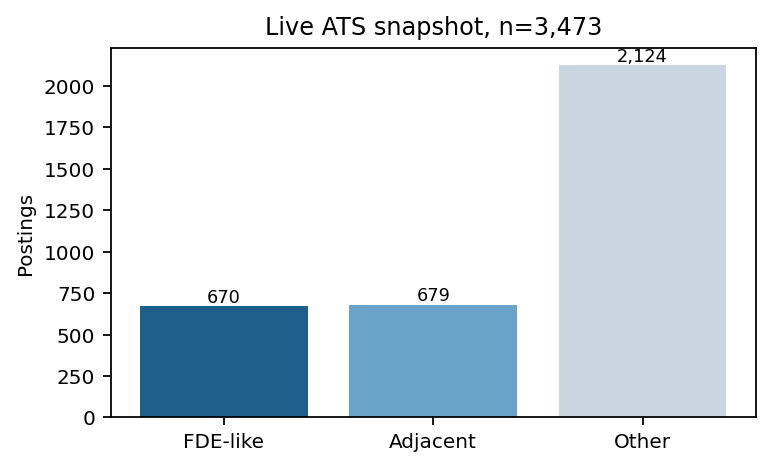
\includegraphics[width=0.48\linewidth]{fig_market_roles.png}
\hfill
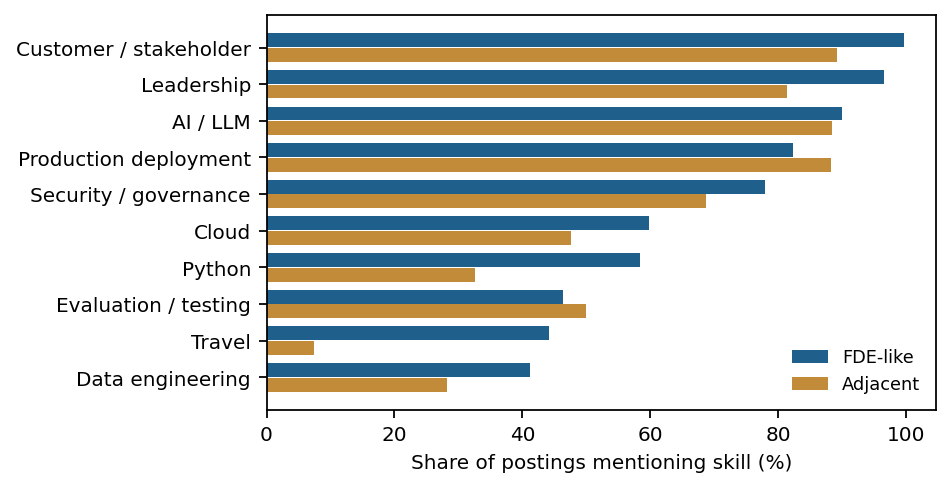
\includegraphics[width=0.48\linewidth]{fig_market_skills.png}
\caption{Live market snapshot. Left: role composition with the broad FDE-like class. Right: skill mentions in FDE-like versus adjacent postings. Absolute shares are upper bounds because ATS boilerplate inflates them.}
\label{fig:market}
\end{figure}

\subsection{Lifecycle difficulty and the verification null}
Table~\ref{tab:benchmark} reports task-resolution rates and partial scores. The ungoverned baseline resolves \ResolveUngoverned{} of tasks. Verification resolves \ResolveVerified{}: across the paired tasks, \VerifiedChanged{} scores changed, \VerifiedImproved{} improved, and \VerifiedWorse{} worsened. \VerifiedIdenticalNonError{} of \VerifiedNonErrorPairs{} non-error pairs were byte-identical; \VerifiedBothError{} additional pairs were both errors. \RepairEpisodes{} verified episodes made a second call. The repair attempt did not move the outcome distribution. The disciplined loop changed \FdeChanged{} of \FdePairs{} paired scores (\FdeImproved{} improved, \FdeWorse{} worsened); \FdeIdenticalNonError{} non-error artifacts were byte-identical to the ungoverned baseline, and \FdeBothError{} pairs were both errors. Across the four policies, the Friedman test gives p = \FriedmanP{}; with template parameterizations we do not interpret it as a population-level test. Partial scores are higher than task-resolution rates, which shows that the model usually produces the right shape and misses one or two controls.

\begin{table}[t]
\centering
\small
\caption{Live FDE-like labor-market snapshot from public ATS boards. Broad and explicit title classes are reported separately.}
\label{tab:market}
\begin{tabular}{ll}
\toprule
Metric & Value \\
\midrule
Postings collected (point-in-time ATS snapshot) & 3,473 \\
FDE-like postings (broad regex class) & 670 (19.3\%) \\
Explicit forward-deployed titles (subset) & 229 (6.6\% of all; 34.2\% of FDE-like) \\
Adjacent postings & 679 \\
Remote share, FDE-like & 24.2\% \\
Median description length & 7,260 chars \\
Postings with a parseable salary mention & 205 (30.60\%) \\
\bottomrule
\end{tabular}
\end{table}

\begin{table}[t]
\centering
\small
\caption{FDE-LifecycleBench results by model and policy. Task resolution and governance compliance are reported separately.}
\label{tab:benchmark}
\begin{tabular}{lllllllll}
\toprule
Model & Policy & n & Task resolved & 95\% CI & Score & Gov. comp. (required) & Saf. viol. & Err. \\
\midrule
qwen2.5:1.5b & ungoverned & 48 & 9 (18.8\%) & [10.2\%, 31.9\%] & 0.592 & n/a & 0 & 2 \\
qwen2.5:1.5b & verified & 48 & 9 (18.8\%) & [10.2\%, 31.9\%] & 0.592 & n/a & 0 & 2 \\
qwen2.5:1.5b & governed & 48 & 16 (33.3\%) & [21.7\%, 47.5\%] & 0.663 & 0/15 & 0 & 1 \\
qwen2.5:1.5b & fde\_disciplined & 48 & 11 (22.9\%) & [13.3\%, 36.5\%] & 0.537 & 0/15 & 0 & 10 \\
\bottomrule
\end{tabular}
\end{table}

\begin{table}[t]
\centering
\small
\caption{Prompt-injection detection on the held-out deepset split.}
\label{tab:guardrail}
\begin{tabular}{lllll}
\toprule
Detector & Precision & Recall & F1 & FPR \\
\midrule
Regex rules & 100.0\% & 3.3\% & 0.063 & 0.0\% \\
TF-IDF + LR @0.5 & 87.0\% & 77.0\% & 0.817 & 6.8\% \\
TF-IDF + LR @target & 65.2\% & 95.1\% & 0.773 & 30.1\% \\
\bottomrule
\end{tabular}
\end{table}

\begin{table}[t]
\centering
\small
\caption{Shadow-price cost model at hosted-equivalent token prices.}
\label{tab:cost}
\begin{tabular}{llllll}
\toprule
Model & Policy & Resolve & Cost/ep. & Cost/resolved & Reviews \\
\midrule
qwen2.5:1.5b & fde\_disciplined & 22.9\% & \$6.47 & \$28.23 & 22 \\
qwen2.5:1.5b & governed & 33.3\% & \$4.70 & \$14.11 & 16 \\
qwen2.5:1.5b & ungoverned & 18.8\% & \$0.59 & \$3.14 & 2 \\
qwen2.5:1.5b & verified & 18.8\% & \$0.59 & \$3.14 & 2 \\
\bottomrule
\end{tabular}
\end{table}


\begin{figure}[t]
\centering
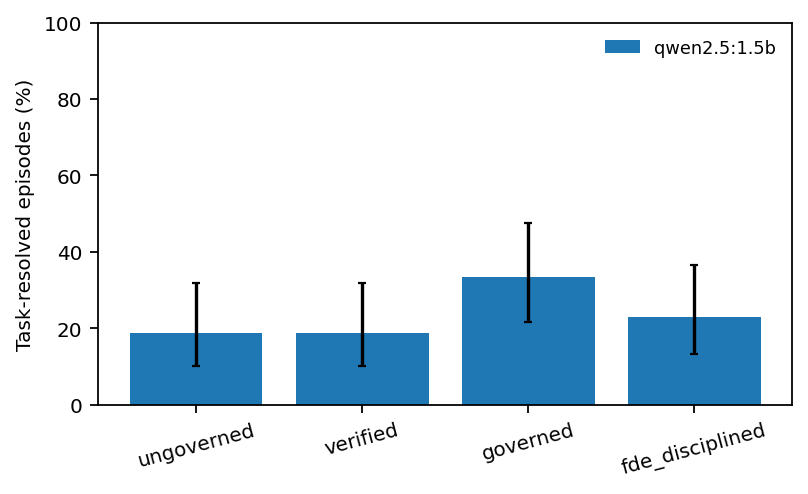
\includegraphics[width=0.62\linewidth]{fig_benchmark_resolve.png}
\caption{Task-resolved episodes by policy with Wilson 95\% intervals. The intervals treat template parameterizations as exchangeable and are optimistic.}
\label{fig:resolve}
\end{figure}

\subsection{Governance is a separate outcome}
Governed task resolution is \ResolveGoverned{} with governance compliance \GovGoverned{} among required high-risk episodes; the instruction alone did not reliably produce approval. The disciplined policy resolves \ResolveDisciplined{} with compliance \GovDisciplined{} among required episodes. \GovHighRiskPerfectUnresolved{} governed or disciplined high-risk episodes passed every task check while omitting the approval field. Calling those episodes ``unresolved'' conflates task quality with governance; calling them ``safe'' ignores the missing approval. The four-policy comparison is therefore descriptive, not a clean causal estimate of governance. The approval requirement is stated in the prompt but is not an acceptance criterion, and the repair feedback never asks for it, so missing approval does not trigger a repair. Inspection of the D01 artifact confirms the confound: the governed run adds the required \texttt{out\_of\_scope} entry while the verified run reproduces the ungoverned artifact; the difference is the prompt bundle, not the approval field.

\subsection{Guardrails}
Regex rules achieve high precision but near-zero recall on the held-out split, because real injections rarely use the exact blocklist phrases. The classifier reaches \GuardRecall{} recall at \GuardPrecision{} precision, with a false-positive rate that is too high for silent blocking but plausible for a review queue. This is the central operational trade-off for an FDE: a detector that misses most attacks creates false assurance, while a detector that flags benign traffic creates review load.

\begin{figure}[t]
\centering
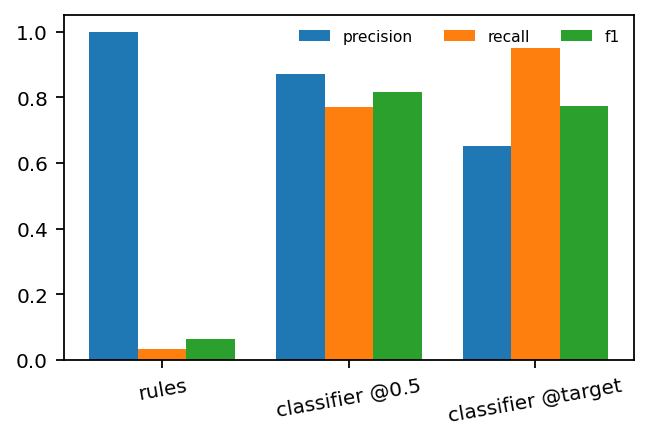
\includegraphics[width=0.52\linewidth]{fig_guardrail.png}
\caption{Prompt-injection detection: rules versus classifier operating points.}
\label{fig:guardrail}
\end{figure}

\subsection{Deployment and cost}
All three canonical stacks reached healthy state. These are infrastructure smoke tests: P01 is an HTTP liveness check; P02 and P03 add dependency and restart checks but do not exercise application logic. Generated artifacts are a stricter test: \DeployValidCompose{} of \DeployTotal{} deployment episodes produced a parsable Compose \texttt{services} mapping. We therefore do not claim that generated stacks run. Human review dominates the cost model at low resolve rates, so cost per resolved task is unstable when the denominator is small. The live Lambda price is \$\LambdaGBSecond{} per GB-second plus \$0.0000002 per request, which makes the serverless control plane negligible relative to engineering time.

\begin{figure}[t]
\centering
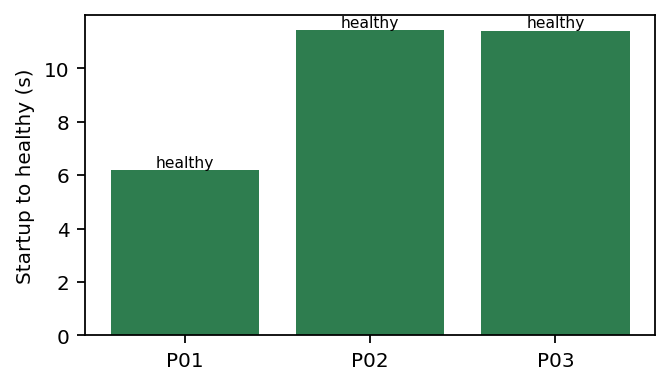
\includegraphics[width=0.48\linewidth]{fig_deployment.png}
\hfill
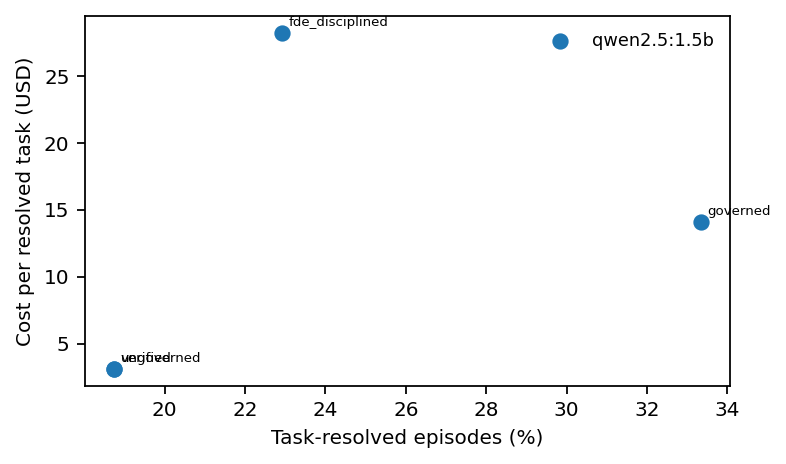
\includegraphics[width=0.48\linewidth]{fig_cost_effectiveness.png}
\caption{Left: canonical deployment startup. Right: cost per resolved task versus task-resolution rate.}
\label{fig:deploycost}
\end{figure}

\section{Discussion}
\paragraph{The null result is the result.} A check-driven repair loop is a natural way to make an FDE agent more reliable, and it is the mechanism behind the \texttt{verified} and \texttt{governed} policies. In this run it changed nothing: the model either already satisfied the checks or could not convert the failure feedback into a passing artifact. The \VerifiedIdenticalNonError{} non-error byte-identical pairs suggest that the second call often repeated the first, and the \RepairEpisodes{} repair attempts did not produce a single score improvement. This is consistent with a small model that is not using the feedback, and with a task bank whose checks are visible and whose failures are often structural (missing keys, wrong types, missing required terms). It is not evidence that verification is useless in general; it is evidence that this implementation and this task bank do not demonstrate a gain.

\paragraph{The disciplined loop is not a free win.} The plan--critique--repair loop changed \FdeChanged{} of \FdePairs{} paired scores, improving \FdeImproved{} and worsening \FdeWorse{}. It also produced \FdeIdenticalNonError{} byte-identical non-error artifacts. A critique step can revise a passing artifact into a worse one, and the current critique prompt has no acceptance gate of its own. This is a design lesson, not a claim that planning or critique is useless.

\paragraph{Task resolution is not governance.} The pre-audit analysis counted a missing approval field as task failure. That made governed policies look worse and obscured the real question: did the artifact do the task, and did the delivery process satisfy the governance requirement? Separating the outcomes yields a more honest picture. High-risk artifacts can be task-perfect and non-compliant at the same time. A production harness should put approval in the acceptance criteria, or model it as a separate gate with an explicit escalation path, and should never report a single ``resolved'' number that hides which construct failed.

\paragraph{Benchmark design.} The \TaskRows{}-row bank is six templates with eight parameterizations. Five phases reuse one instruction. This is enough to exercise validators and to expose structural failures, but it is not enough to estimate phase difficulty or policy effects across a population of FDE tasks. A credible follow-up needs distinct scenarios per row, hidden or held-out checks, multiple models, repeated runs, and cluster-robust intervals. It also needs tasks where the acceptance criteria are not shown to the model, otherwise the benchmark measures rubric-following rather than capability.

\paragraph{Market measurement.} The broad FDE-like class is a regex construct; the explicit subset is a sensitivity check. Reporting only the broad count would overstate the role's prevalence, and reporting only the explicit count would understate it. The salary heuristic is useful for describing posted ranges but is not a compensation estimate.

\paragraph{Deployment claims.} Canonical smoke tests answer a narrow question: can the harness start a known-good stack, observe health, restart it, and tear it down? They do not answer whether a model-generated stack works. The generated-artifact parse rate is the relevant measurement for that question, and it is low. We report the scope rather than converting a smoke test into a deployment claim.

\section{Threats to validity}
\paragraph{Template structure.} The benchmark has \TaskRows{} rows but only \TaskTemplates{} templates and \DistinctInstructions{} distinct instructions. Rows within a phase are parameterizations, not independent scenarios. Confidence intervals and paired tests treat them as exchangeable and are therefore optimistic.

\paragraph{Rubric leakage.} The model sees the acceptance criteria. High scores measure instruction-following against visible checks, not hidden FDE capability.

\paragraph{Model scale.} The reported run uses a 1.5B model. Results characterize this model and task bank, not frontier systems.

\paragraph{Single deterministic run.} Each cell is one episode at temperature zero. There is no estimate of run-to-run variance, and the paired tests do not account for model or prompt sampling.

\paragraph{Governance confound.} \texttt{requires\_human\_approval} is outside the task checks. Governed and disciplined policies are not clean estimates of the causal effect of approval, and the repair feedback never asks for approval.

\paragraph{Market sample.} ATS boards over-represent AI-native companies. The broad FDE-like class is a regex construct; the explicit subset is a sensitivity check, not a ground truth. Salary parsing is heuristic and may include OTE or non-base figures.

\paragraph{Guardrail corpus.} deepset is small, English-heavy, and older than the 2026 threat landscape. The 95\% recall point has a high false-positive rate. Results should be re-estimated on customer traffic before deployment.

\paragraph{Deployment environment.} Canonical smoke tests use cached images and a local Docker daemon. Generated artifacts were parsed but not executed. Registry policy, Kubernetes, and multi-tenant isolation are out of scope.

\paragraph{Cost model.} Token prices are shadow prices; the local run has no per-token bill. Human review time is an assumption, not a measurement.

\section{Ethics and data}
We use public job postings and public research datasets. We do not collect customer data, credentials, or personal information. Prompt-injection examples are public and used only for detection research. Deployment tests run locally and are destroyed after each episode. The benchmark is intended to improve the safety and reliability of enterprise deployments, not to automate the displacement of the engineers who do them.

\section{Conclusion}
FDE work is growing faster than the evidence about it. This paper contributes a point-in-time market snapshot, a six-template benchmark with explicit acceptance criteria, a four-policy measurement, a guardrail evaluation, a canonical-only deployment smoke test, and a cost model. The headline is a null result: one check-driven repair attempt changed none of the paired scores, and task resolution must be reported separately from governance compliance. The task bank, harness, freeze manifest, and generated artifacts are released so that the claims can be checked, extended, and falsified.

\bibliographystyle{plainnat}
\bibliography{references}

\appendix
\section{Task bank structure}
The full bank is in \texttt{data/benchmark/tasks.json}, generated by \texttt{python -m fde\_research.tasks}. Each row contains its brief, evidence, instruction, checks, and reference artifact. The validator is in \texttt{src/fde\_research/validators.py}; reference self-validation runs in CI. The bank has \TaskRows{} rows, \TaskTemplates{} phase templates, and \DistinctInstructions{} distinct instruction strings.

\section{Reproduction commands}
\begin{verbatim}
make tasks
make market
make benchmark
make guardrail
make deployment
make cost stats figures
make report
make verify
\end{verbatim}

For the reported analysis, the benchmark is frozen first:
\begin{verbatim}
PYTHONPATH=src python -m fde_research.freeze_run --label final
FDE_EPISODES=results/frozen/benchmark_episodes_final.jsonl \
  make cost stats figures report verify
\end{verbatim}

\end{document}
